	
\documentclass[review]{elsarticle}
\usepackage{hyperref,lineno}
\usepackage{xcolor}
\usepackage[utf8]{inputenc}
\modulolinenumbers[5]

%\newcommand{\memo}[2]{\textcolor{#1}{#2}}
%\newcommand{\maria}[1]{\memo{red}{#1\\}}
%\newcommand{\revise}[1]{\memo{blue}{#1\\}}

\journal{Journal of Archaeological Science}


\bibliographystyle{model2-names.bst}\biboptions{authoryear}


\begin{document}

\begin{frontmatter}

\title{Identifying social learning between Roman amphorae workshops through morphometric similarity}


\author[bscadress]{Maria Coto-Sarmiento\corref{mycorrespondingauthor}}
\cortext[mycorrespondingauthor]{Corresponding author}
\ead{maria.coto@bsc.es}


\author[edadress]{Xavier Rubio-Campillo}
\author[ceipacadress]{Jos\'e Remesal}


\address[bscadress]{Barcelona Supercomputing Center (BSC), Jordi Girona 29, Office 3A, Nexus II Building, 08034, Barcelona, Spain}
\address[edadress]{School of History, Classic \& Archaeology, Room OOM.33, William Robertson Wing, Old Medical School, Teviot Place, University of Edinburgh, UK}
\address[ceipacadress]{CEIPAC, Department of Prehistory and Archaeology, Montalegre, 6-8, 08001, University of Barcelona, Barcelona, Spain}

\begin{abstract}

The aim of this study is to interaction interactive dynamics within amphorae workshops in the Roman Empire. The Baetica province (currently Andalusia, southern Spain) hosted for almost 300 years a massive infrastructure that supplied olive oil to the Western provinces of Rome. A large number of workshops produced the same type of amphora to ship the product through maritime and riverine transport networks. Despite the amount of evidence it is difficult to find an archaeological proxy able to tell us how these workshops were organised.

We apply here an evolutionary framework to understand potential links between workshops through morphometric similarities in the amphorae they produced. By exploring small yet statistical significant differences in the amphorae made in 5 different workshops the approach is able to identify how individual potters acquired and transmitted technical skills.  Our approach applies multivariate statistical methods to cluster a variety of amphorae based on morphometric measurements. Other studies have developed similar approach to analyse handmade pottery but we show here that the method can be also applied to large-scale production of a standardized amphora type (i.e. Dressel 20).

Results suggest that morphometric similarity is inversely correlated with spatial distance between workshops. This outcome suggests that pottery-making techniques were transmitted through oblique transmission with little or no movement of potters between distant workshops.

The work also highlights that morphometric similarity may be an effective proxy to identify social learning dynamics even amongst workshops producing exactly the same amphoric type. 

\end{abstract}

\begin{keyword}
Roman Empire; amphorae workshops; Dressel 20; social learning; cultural evolution
\end{keyword}

\end{frontmatter}

\linenumbers

\section{Introduction}

The archaeological record can help us identify the mechanisms by which humans learn from each other~\citep{richerson2005not,eerkens_jelmer_cultural_2007}. Cultural transmission dynamics can be identified by analysing archaeological proxies able to capture the distinct variability generated by different social learning mechanisms~\citep{shennan_ceramic_2001,eerkens_jelmer_cultural_2005, gandon_copying_2014}. This approach has been successfully applied to the material culture generated by small-scale societies but it has been seldom explored in the case of large-scale production~\citep{shennan_isolation-by-distance_2015}.

This paper explores the social dynamics of specialized production in the Roman Empire. We focus here on analysing large-scale production of a single amphoric type (Dressel 20) in a specific area. An evolutionary framework is used to identify social learning dynamics between pottery-makers \citep{shennan_evolution_2008,mesoudi_cultural_2015}. 

Following a large number of authors \citep{neff1992ceramics,shennan_genes_2002,bowser_learning_2008,hosfield_modes_2009}, pottery production can be learned by different modes of cultural transmission depending on the level of production in the communities. Vertical transmission is a mode of transmission whose teaching of the production is done from parents to offspring (biological transmission); oblique transmission from master to young generation of disciples while in horizontal transmission individuals teach pottery techniques to other individuals within the same level and those workers spread the knowledge to their community \citep{cavalli-sforza_cultural_1981, acerbi_cultural_2006}

Artefact variation should also be affected by geographical distance \citep{bjorklund_effect_2010,shennan_isolation-by-distance_2015, van_strien_isolation-by-distance_2015}. If vertical or oblique transmission are predominant then material culture should be similar in nearby groups with high degree of interaction \citep{hart_effects_2012}. The underlying consequence is that it should be possible to identify interaction between workshops by quantifying similarity amongst the amphorae they produced; if apprentices moved between distant workshops then no differences would be found on this proxy while a more strict oblique transmission would be revealed by distant workshops exhibiting less similarity.

The debate on social learning processes is hindered by the challenge of detecting the different modes of transmission in the archaeological record \citep{roux_standardization_2015}. In the case of archaeology, several studies have analysed this process focused on the production of handmade pottery \citep{steele_james_ceramic_2010} or with stylistic variations \citep{neiman_stylistic_1995, shennan_ceramic_2001}. Our work aims at identifying learning processes even in the case of the standardized massive olive oil production common during the Roman
Empire \citep{bevan_mediterranean_2014}. 

Olive oil was one of the most important products of the Classical Mediterranean world as it was used in almost all aspects of daily life including cooking, lightning and hygiene \citep{mattingly_d.j._oil_1988}. The Baetica province (currently Andalusia, southern Spain) developed a massive infrastructure of olive oil production to face the demands of the Roman Empire. The product was shipped in large amounts of amphorae to distant provinces all along the Western provinces. One of its most important clients was the Roman army as olive oil was supplied to tens of thousands of legionaries in places such as Britannia \citep{monfort_britannia_1998,funari_economic_2005} and Germania \citep{remesal_annona_1986}. 

For this reason, this ancient province became an important support for the production and distribution of olive oil to the rest of the Empire during three centuries \citep{millet_anforas_1998, rodriguez_baetican_1998,chic2005comercio}. Baetica provided a strong connectivity through riverine transport that allowed inland producers to use an important trade network through the Mediterranean and Atlantic \citep{garcia_vargas_enrique_formal_2010}. The exponential production growth required the creation of over a hundred amphora workshops supporting olive oil shipment. These workshops were located along the Guadalquivir river and its tributaries. The majority of amphorae produced in this area are classified as Dressel 20 type divided into a variety of subclasses \citep{martin-kilcher_romischen_1994,berni_millet_epigrafianforica_2008}. Dressel 20 was used mostly to transport olive oil for around 300 years in order to satisfy the demand within Roman Empire \citep{rodriguez_economioleicola_1977}. 

The question about the organization of potters within Roman Empire remains under discussion due to the lack of archaeological and written evidences. Several studies have analysed amphorae using a diversity of approaches, from chemical analyses to large-scale distribution \citep{isaksen_network_2006,brughmans_roman_2016,coto-sarmiento_maria_bayesian_????}. However, the structure of social learning that transmitted knowledge on how amphorae were made is still poorly understood. It still remains unknown whether these workshops were run by families or groups of owners without kinship. Did they have different traditions and apprentices worked in the place where they were trained? Did potters work in more than one workshop? Were changes in production decided by workshops or by external actors? All these questions are linked to the social learning processes that took place in the workshops. On the other hand, archaeological record shows this specialized production as highly organized both in terms of products and processes and with apparently few variations. The same type of amphorae was produced over 300 years while similar stamps and information was recorded on them \citep{remesal_anforas_2004}.

If the system was organised based on oblique transmission mechanisms with no potters moving to distant workshops then amphorae produced in nearby workshops might share more similar traits than with the rest of the production. On the other hand, if horizontal dynamics were common then this correlation with spatial coordinates should not be present as workers would share their methods

The paper can be summarized as follows. The next section introduces the dataset and the methods used to analyse it. Section three presents the results while the last part discusses the outcomes and highlights the main conclusions of the work. 

\section{Material and methods}

\subsection{Workshops}

Our sample consisted of 413 Dressel 20 amphorae collected from the 5 Dressel 20 workshops that have been more intensively excavated in the last decades. The workshops were located at Malpica, Cerro del Belén (hereafter, Belén) \citep{diaz_trujillo_excavacion_1992}, Parlamento \citep{garcia_vargas_anforas_2000}, Villaseca\citep{garcia_vargas_enrique_excavacion_????} and Las Delicias \citep{fernandez_excavacion_2001,_atelier_2014} (see Figure \ref{romanworkshop}).

\begin{figure}[htp]
	\centering
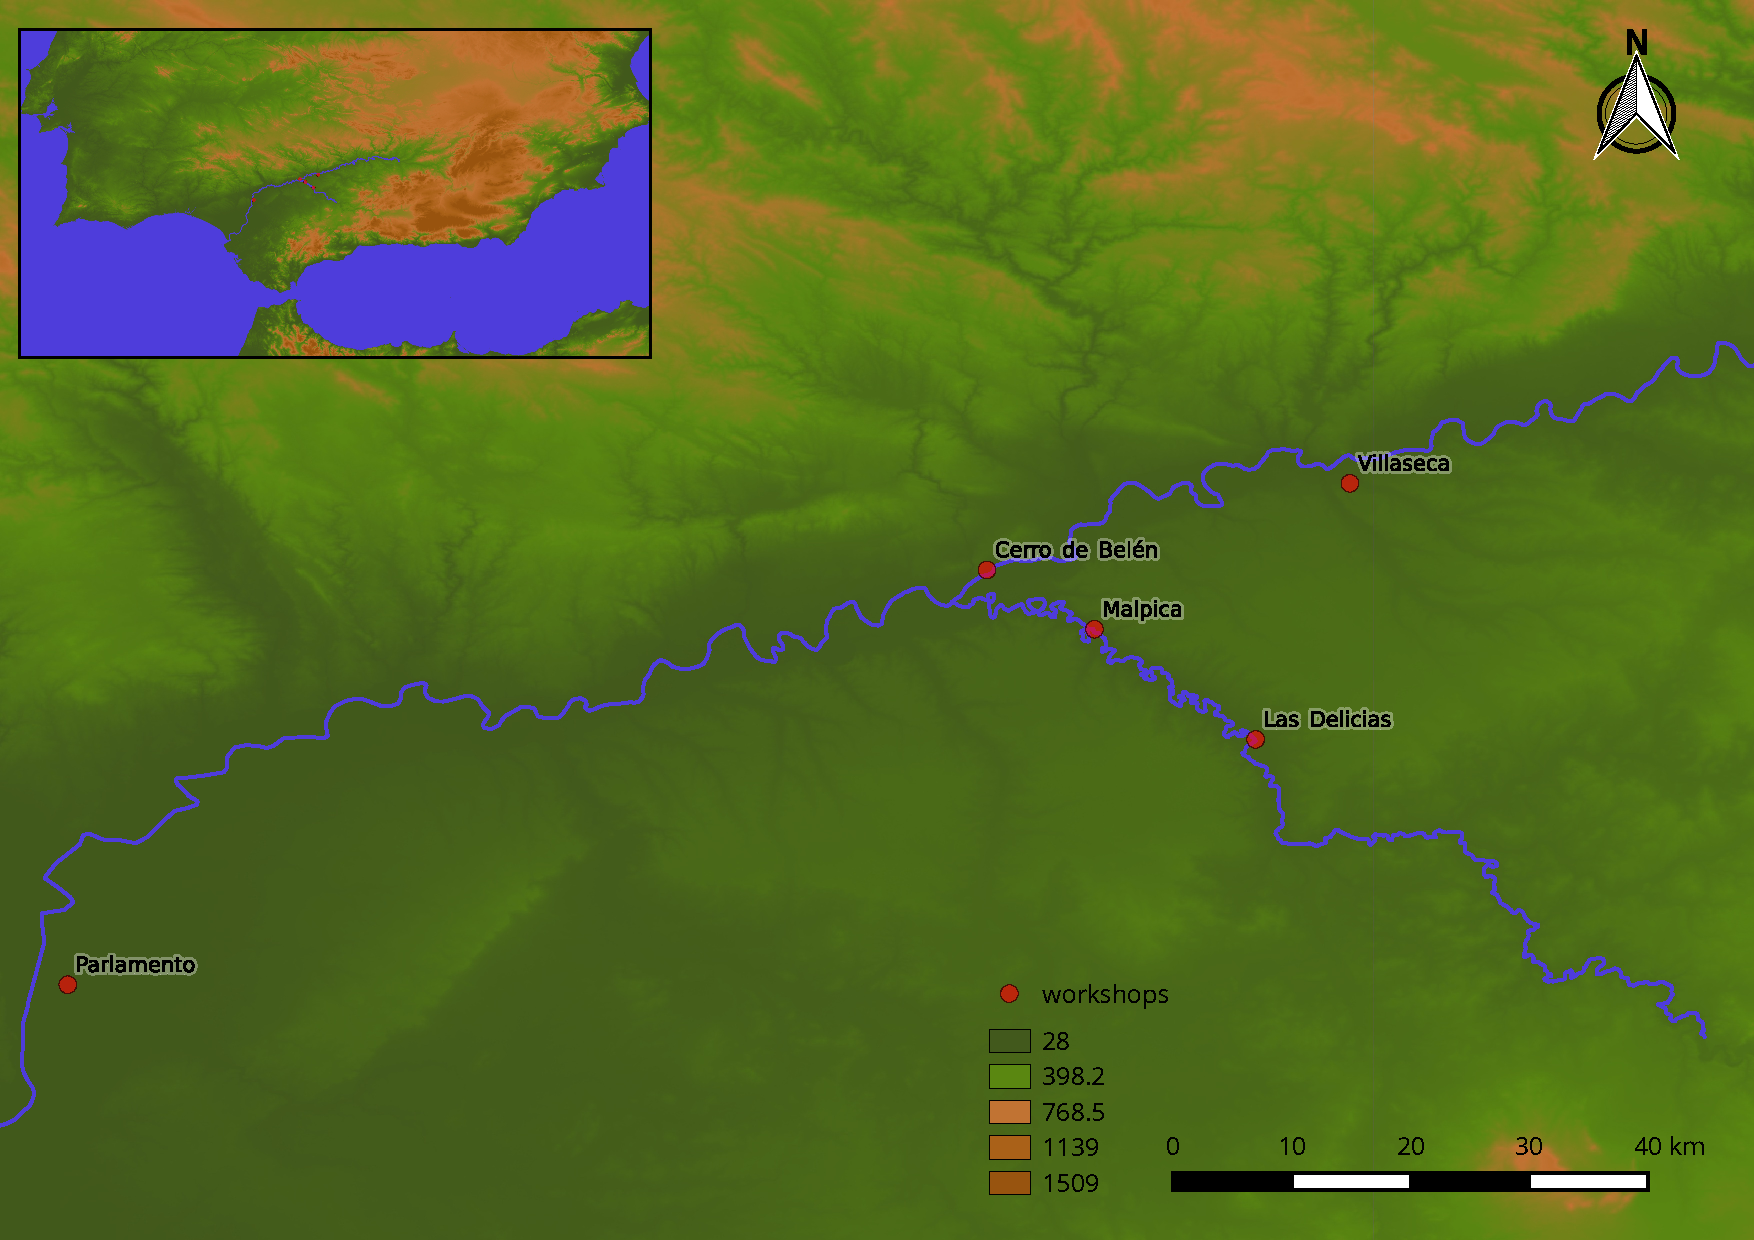
\includegraphics[width=\linewidth]{figs/romanworkshop}
\caption{Map from Baetica province during the Roman Empire depicting the location of the 5 analysed workshops. Dressel 20 workshops were mostly distributed along the rivers Gualdalquivir and Genil.}
\label{romanworkshop}
\end{figure} 

The sample was roughly uniformly distributed amongst the 5 workshops (80-100 samples for each of them). These workshops were distributed in a diversity of locations therefore spatial dynamics could be potentially identified. All of them had long work activity so differences in amphorae could display overlapping temporal variation. 
This trait is reinforced by the fact that the Dressel 20 type remained almost unchanged over three centuries \citep{berni_dressel_2016}. We analysed Dressel 20 of the three most abundant variants in our dataset spanning approximately three centuries (Dressel C, Dressel D, Dressel E) \citep{martin-kilcher_romischen_1994,berni_millet_epigrafianforica_2008}. All the variants were found in the 5 workshops so no intrinsic bias was generated by them. 

\subsection{Spatial Distance}

The approach required us to compute a pairwise matrix of spatial distances between workshops. All these workshops were located near a river as the amphorae were shipped by boat after being made and filled with olive oil. Given the relevance of riverine transport it was decided that the best proxy for spatial distance between workshops was the one observed following the river course, as summarized in Table~\ref{table:distances}

\begin{table}[htp]
\centering

\begin{tabular}{lccccc}
\hline

\textbf{Workshops} & Malpica & Belén & Villaseca & Las Delicias & Parlamento \\ \hline
Malpica & - & 11 & 50 & 17 & 108 \\
Belén & 11 & - & 33 & 29 & 98 \\
Villaseca & 50 & 33 & - & 67 & 133 \\
Las Delicias & 17 & 29 & 67 & - & 126 \\
Parlamento & 108 & 98 & 133 & 126 & - \\
\hline
\end{tabular}
\caption{Distance matrix between workshops (in km.)}
\label{table:distances}
\end{table}

\subsection{Measurements}

Eight different measurements were taken from each amphora. The metrics were focused on the rim sherds as this section presents the best preservation for most archaeological contexts and they present good indicators of variation \citep{berni_millet_epigrafianforica_2008}. Other interesting proxies such as handles and bases were found in lesser quantities and for this reason they would be less appropriate for quantitative approaches due to low sample size. The measurements can be seen in Figure~\ref{mesures}; they were divided into exterior diameter, inside diameter, rim height, rim width, shape width, rim inside height, rim width 2 and protruding rim.

\begin{figure}[htp]
	\centering
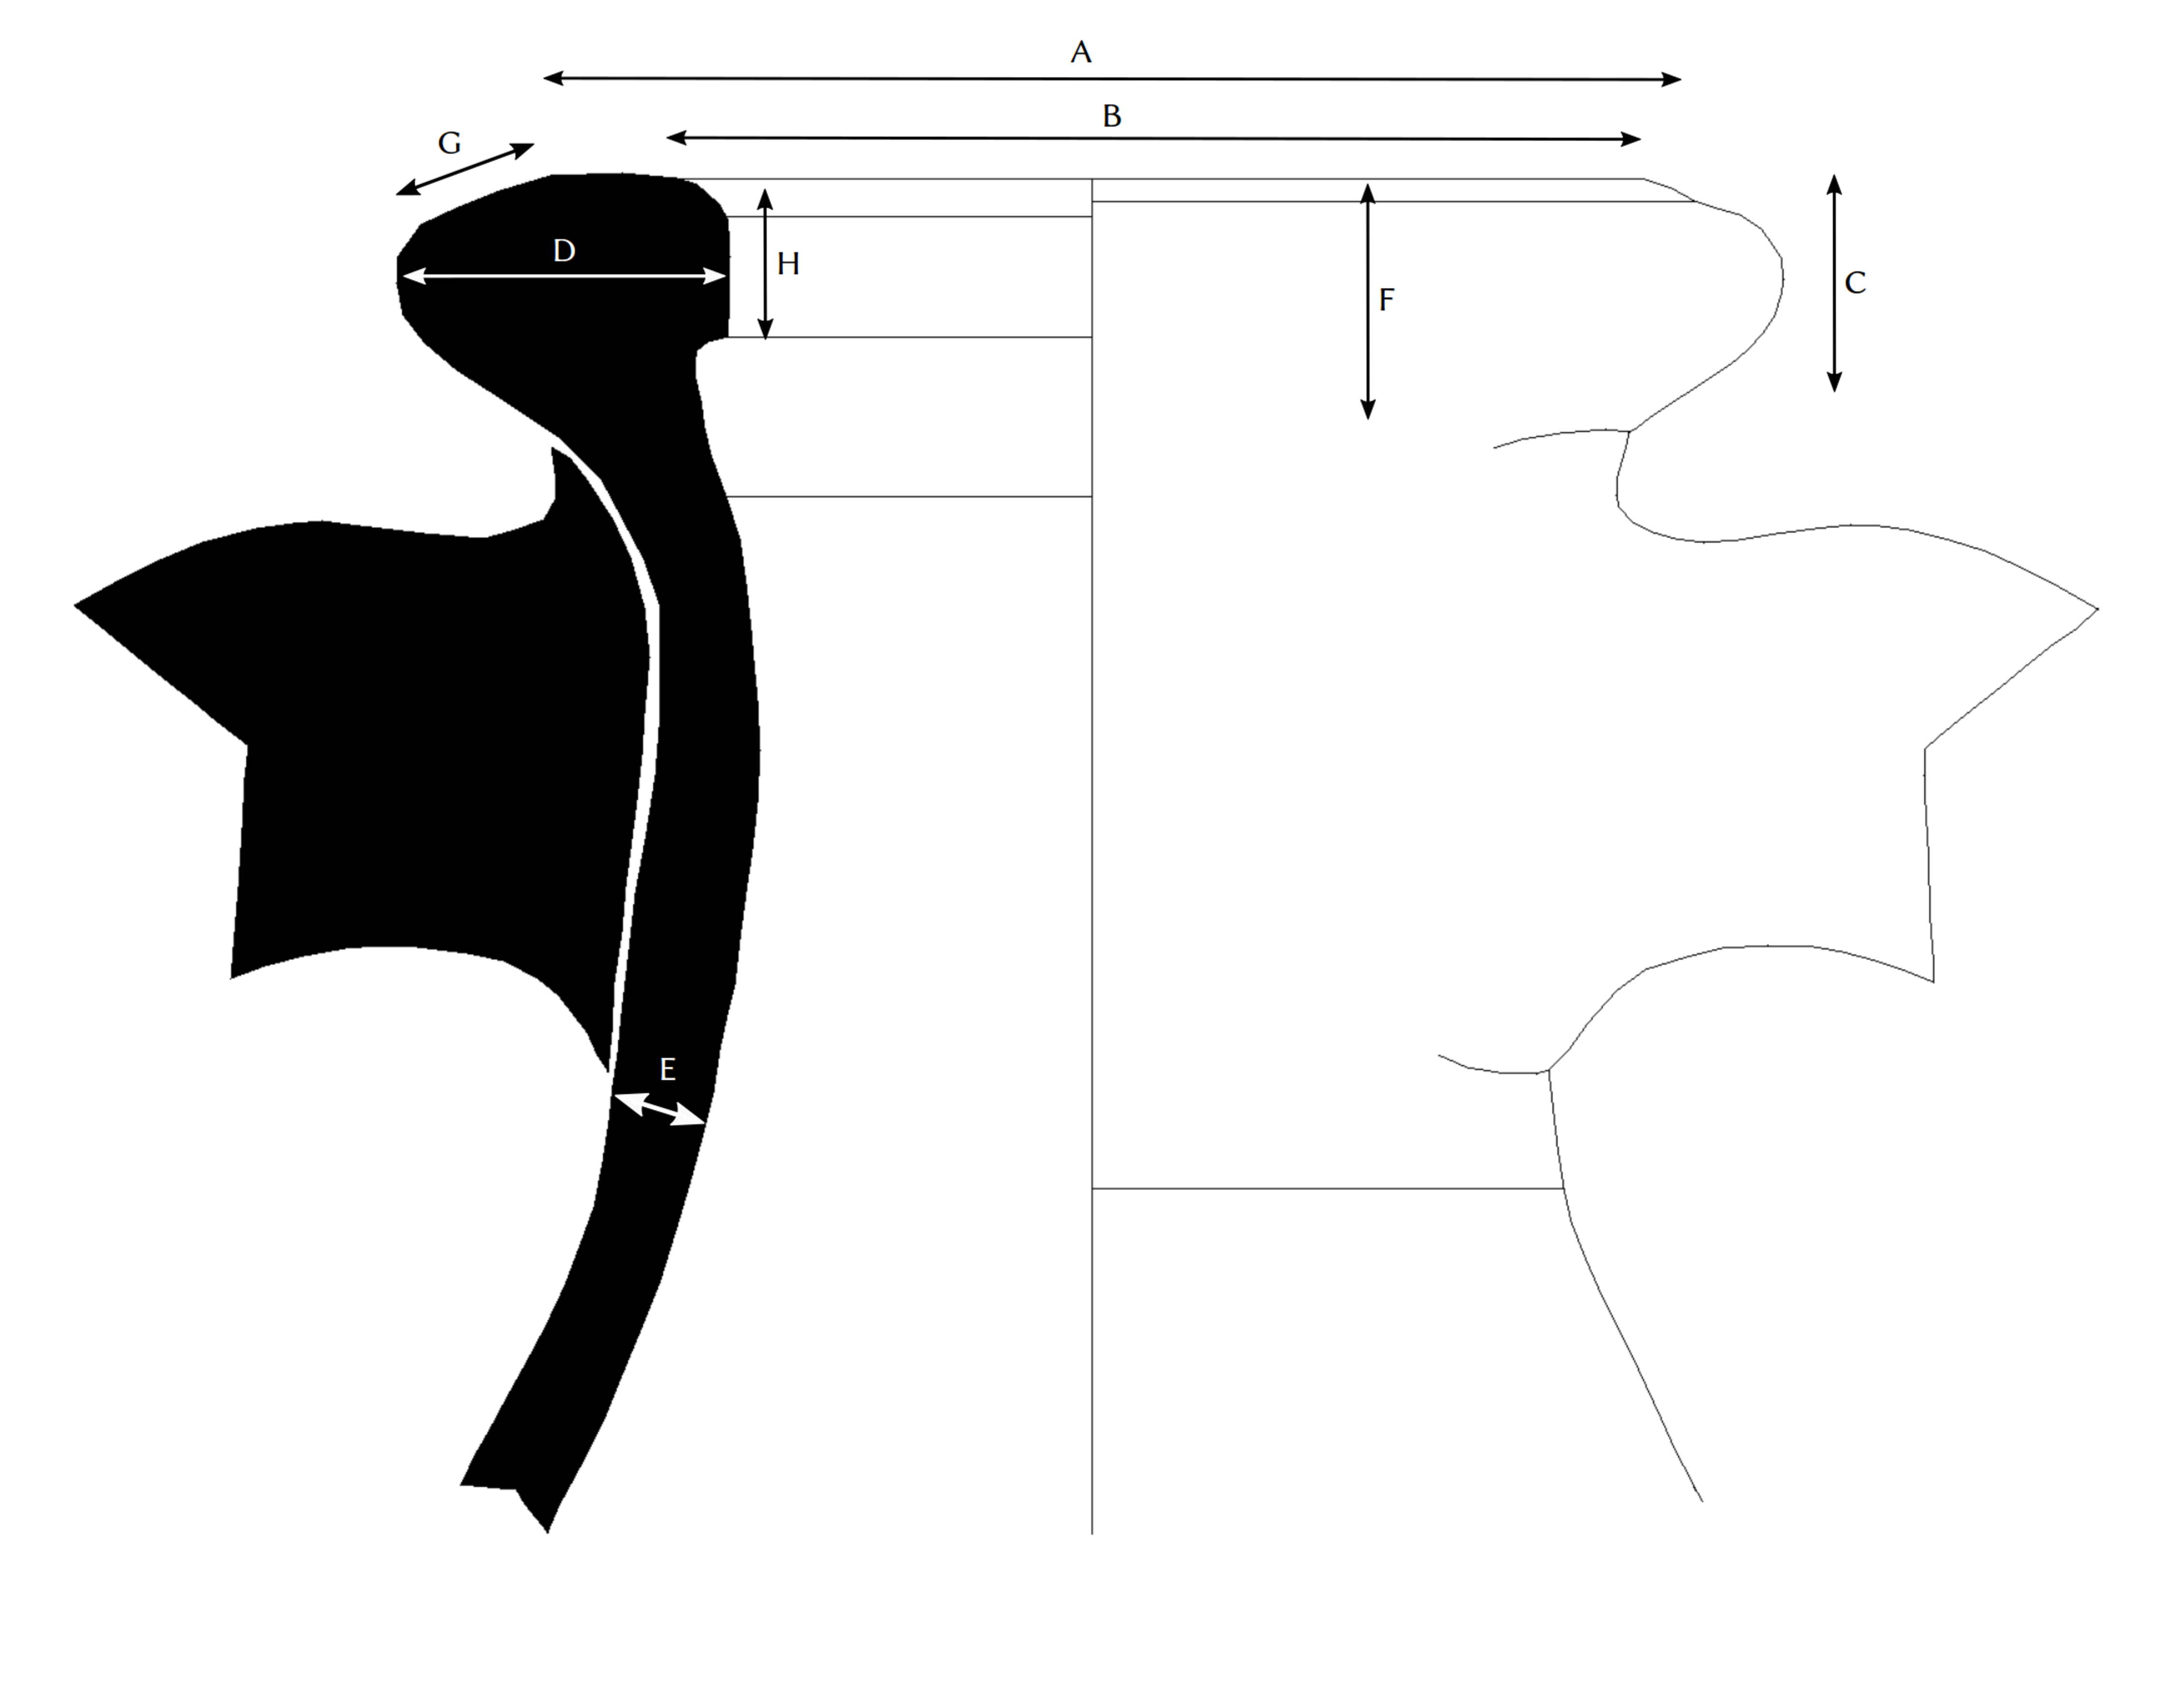
\includegraphics[width=\linewidth]{figs/mesures.pdf}
\caption{The 8 morphometric measurements taken for all amphorae. A: External diameter. B: Inside diameter. C: Rim height. D: Rim width. E: Shape width. F: Rim inside height. G: Rim width 2. H: Protruding rim}
\label{mesures}
\end{figure} 

\subsection{Exploratory Data Analysis}

Principal Component Analysis (PCA) was used to explore the variation of measurements over the different workshops \citep{jolliffe_principal_2002} . PCA is a common method in archaeology in scenarios studying within-sample variation \citep{shennan_quantifying_1997, li_crossbows_2014, schillinger_differences_2016}.The method allowed us to visualize the dataset by focusing on a small number of Principal Components (PCs) while retaining a majority of the variation which was in essence what we wanted to explore. 

\subsection{Morphometric similarity} 

Exploratory Data Analysis was followed by the measurement of pairwise dissimilarity between the amphorae made in different workshops. The approach presented here is based on the idea that if most amphorae made in two workshops are difficult to distinguish then the workshops are making similar artefacts; on the other hand if the probability of distinguishing the production place of most amphorae is high then there are remarkable morphometric differences between the objects. This goal could be achieved by 1) training a clustering algorithm with the dataset 2) using the model to predict the workshop of the same dataset and 3) computing a confusion matrix.

The choice of clustering method was Linear Discriminant Analysis (LDA). The entire dataset was used both for the training and prediction steps as we were interested on how well workshop attribution could be predicted relying exclusively on morphometric measures. A Confusion Matrix was then computed as a quantification of the extent to what amphorae of different workshops can be identified. The Confusion Matrix computes this quantity as the number of misclassifications between each pair of groups in the dataset (i.e. the workshops). This method has already been used in similar scenarios aiming at identifying differences in artefact production \citep{thorpe_distribution_1984,i_martin_alisis_1998,charlton_investigating_2012}. If the amphorae made in two workshops were easily confused then their average measures must be similar; on the other hand, if the rate of misclassification between two workshops is very low then the amphorae made in these locations are distinctively different.

The diagonal of the confusion matrix (i.e. correct classifications) was removed and the number of confusions per each workshop was then divided by the total number to get the percentage of errors from a given workshops to the rest of the sample. These values were finally normalized to generate a pairwise distance matrix of morphometric measurements.

\subsection{Dissimilarity correlation}

The last step of this method was the comparison of morphometric and spatial distance matrices. A significant correlation between these dissimilarity matrices would suggest processes of isolation-by-distance typical from oblique transmission.

The evaluation of these two distance matrices (morphometric distance and spatial distance) was computed using a Mantel test. Mantel test evaluates the degree of pairwise correlation between two matrices and has been particularly useful in archaeology to explore the spatial dimension of cultural change \citep{mantel_detection_1967, diniz-filho_mantel_2013, crema_culture_2014}.  

\section{Results}

\subsection{Principal Component Analysis}

The loadings for the two main Principal Components of the dataset are listed in Table~\ref{table:pca}

\begin{table}[htp]
\centering
\begin{tabular}{lcccccccc}
\hline
Variables & PC1 & PC2 \\ \hline
Exterior diameter & 0.877 & 0.312 \\
Inside diameter & 0.404 & -0.887 \\
Rim height & - & - \\
Rim width & 0.149 & 0.119 \\
Shape width & - & - \\
Rim inside & - & - \\
Rim width 2 & 0.133 & 0.142 \\
Protruding rim & -0.159 & -0.272 \\
\hline
\end{tabular}
\caption{Two main Principal Components. Diameter values and the protruding rim seem to capture the majority of variation.}
\label{table:pca}
\end{table}

A exploratory visualization for these two main Principal Components can be seen in Figure \ref{pca}. The plot suggests that each workshop exhibits slightly different dynamics for PC1 while PC2 is distinctively different for the two most distant sites (Villaseca and Parlamento). Additionally, the first PC also tends to display more similar values for amphorae made in nearby workshops such as Bel\'en and Malpica. The exploratory analysis was also tested individually by Dressel 20 types in order to observe differences according to the chronology. A similar pattern is observed in Figure \ref{dressel}. The result suggests  a noticeable variability between Dressel C and Dressel D and E but barely perceptible between Dressel D and E.

\begin{figure}[htp]
	\centering
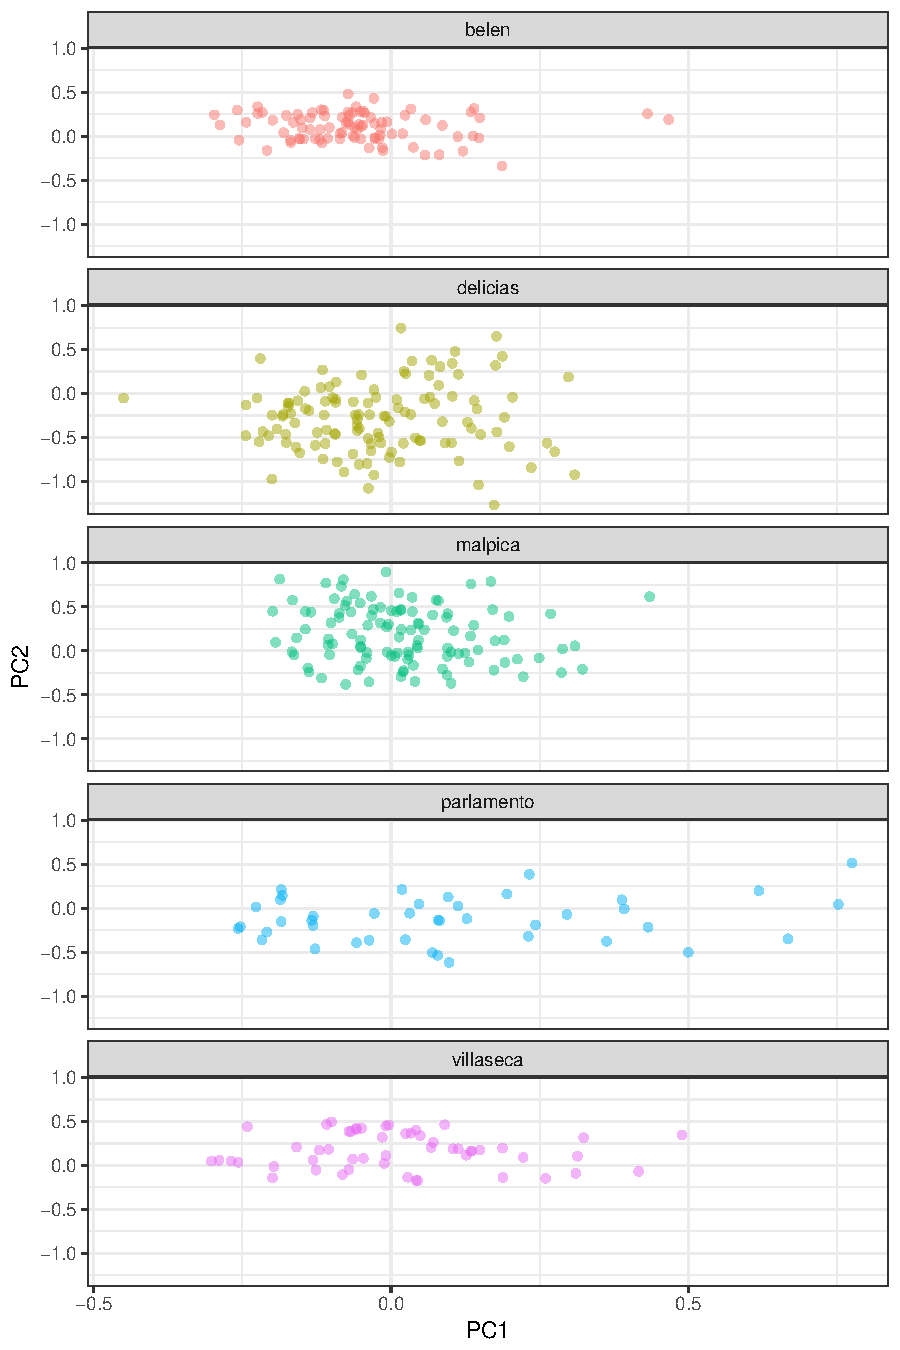
\includegraphics[width=\linewidth]{figs/pca}
\caption{Scatter and density plot for the First and Second PCs. Sample is split by workshop}
\label{pca}
\end{figure} 


\begin{figure}[htp]
	\centering
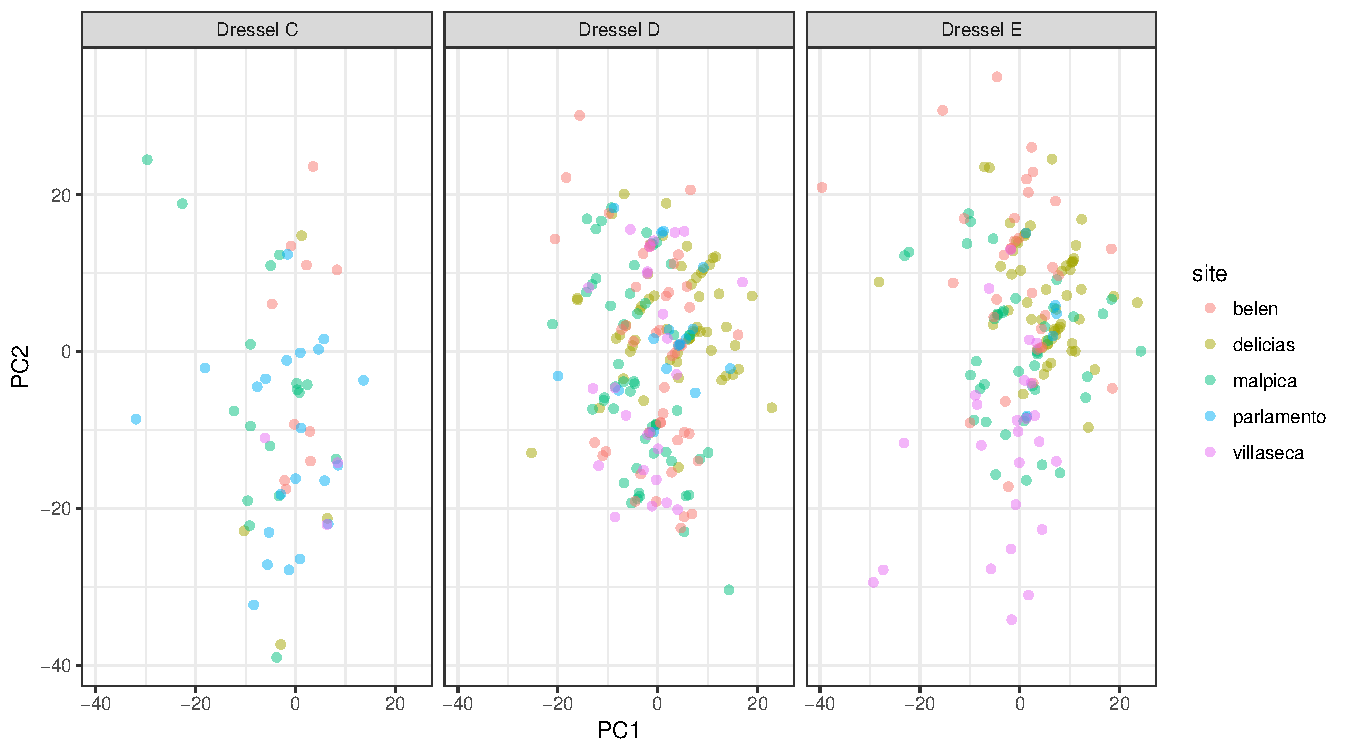
\includegraphics[width=\linewidth]{figs/dresseltypes}
\caption{Scatter plot for the First and Second PCs. Sample is divided by Dressel 20 types}
\label{dressel}
\end{figure} 


\subsection{Linear Discriminant Analysis}

LDA's prediction generated an accuracy of 56.6\%. For this method the accuracy of the clustering algorithm is not as relevant as the distribution of errors which can be seen in the Confusion Matrix of Table~\ref{table:confusion}.

\begin{table}[htp]
\begin{tabular}{lccccc}
\hline
      & Belén & Delicias & Malpica & Parlamento & Villaseca\\ \hline
Belén & 48 & 11 & 16 & 4 & 6 \\
Delicias & 10 & 81 & 24 & 8 & 0 \\
Malpica & 12 & 12 & 49 & 1 & 6 \\
Parlamento & 6 & 10 & 9 & 25 & 10 \\
Villaseca & 12 & 5 & 13 & 4 & 31 \\
\hline

\end{tabular}
\caption{Confusion Matrix of errors in predicted classifications between workshops. The sample analysed gave an accuracy percentage of 56.6\% with p-value $<$0.01. }
\label{table:confusion}
\end{table}

A tentative glance to these results suggest that workshops with a minor spatial distance such as Malpica, Belén and Las Delicias made amphorae that are more difficult to distinguish due to their similarity. By contrast, workshops as Parlamento shows a minor misclassification coinciding with a higher spatial distance. 

\subsection{Mantel correlation test}

Mantel test between morphometric and spatial dissimilarity matrices generated a correlation of $0.51$ with p-value under $0.01$. The analysis shows that morphometric distance of the amphorae are strongly correlated with the spatial distance of workshops. Accordingly closer workshops tend to be more similar than the rest: when geographic distance is low, as the example of Belén and Malpica, the morphometric distance seems more similar whereas when distance is higher, as Parlamento, the morphometric distance displays differences with the rest of workshops. Thus, the results suggest that the variability on the making-techniques processes might depend on the spatial distance.   

\section{Discussion and Concluding remarks}

Similarity on the making techniques processes among workshops shows a inverse correlation with spatial distance. The analysed morphometric traits suggest that the similarity between amphorae decreases with the spatial distance between the workshops where they were produced. As a result, amphorae made in nearby workshops share more similar traits than amphorae made in distant workshops where contact was less frequent. 

Horizontal transmission or high mobility do not seem to match with the results of the analysis. Scenarios with frequent contact between potters or workers moving from workshop to workshop would have generated larger homogeneity in the technical practises with low intensity of isolation-by-distance processes. As a consequence workshops sharing a network of potters would have employed the same production techniques, thus generating similar amphorae. The fact that isolation by distance can be identified suggests limited mobility strictly linked to nearby workshops.

The variability on the morphological techniques between workshops does not suggest different modes of production techniques of making amphorae. Neither any intentionality of modification or improvement of these techniques has been detected in the analysis. 

Rather the results suggest that oblique transmission could be the main cultural mechanism to explain the variability between workshops. The different morphological traits among workshops seem to reveal low frequency of contact between potters from other workshops. The equilibrium of this dynamic for a long time span (over three centuries) can be interpreted as a high-fidelity social learning mechanism transmitted within each one of the workshops \citep{schillinger_copying_2016}. 

From our perspective, the cause of this variability could have been the consequence of this isolation of pottery workshops over time. In other words, individuals would have copied the same model of amphora from other individuals but unintentionally making small random errors in a same workshop. Hence, each workshop would produce the same amphora assemblages with different mutations caused by accumulating copying error transmitted by generations. The disciples could have remained working at the same workshops where they were trained. These differences seem less remarkable when the production increases in order to satisfy the demand of the Roman Empire, then it tends to be more standardized. 

Despite these results the diversity of social learning processes is always complex. The transmission of technical skills during apprenticeship (master to disciples) and their limited mobility does not imply that horizontal transmission did not exist. It can be a mechanism where this process was initially lead by master to disciples in the same workshops but consequently this transmission would be affected by the high demand of production promoting workers moving to other workshops and exchange ideas. 

To conclude, the method presented here provides a framework to identify social learning mechanisms between production centres based on morphometric measurements of artefacts. The method has proven valuable even in the case of the highly standardized amphoric production of the Roman Empire. The suggested method could also offer a good comparison with other analytical methods such as archaeometry; we believe that a framework integrating and comparing multiple sources of evidence could be extremely effective on the process of characterization of production sites and places of consumption. Our analysis provides a useful guideline for the exploration of the social learning processes connected with amphora production in the Roman Empire. Hence, the results have lightened to understand the link between social learning and archaeological evidence in a diversity of scenarios. 
 

\section{Acknowledgments}

The research was funded by European Research Council Advanced Grant EPNet (340828). We are grateful to Enrique Garc\'ia Vargas, Simon Carrignon, Juan Moros for their useful comments and the two anonymous reviewers and editor for helpful suggestions and constructive comments on previous versions of the paper. The Museum of \'Ecija (Antonio Fern\'andez Ugalde), Museum of Palma del R\'io (Reyes Lopera and Emilio Navarro), Museum of C\'ordoba and Museum of Seville for kindly allowing us access to their information. Data were collected, performed and analysed in R version 3.2.4. statistical language and implemented with the package MASS and vegan. Map was done by QGIS 2.18.15 'Las Palmas' with SRTM data Version 4.1 from CIAT-CSI SRTM website (http://srtm.csi.cgiar.org) \citep{SRTM}. 


\section*{References}

\bibliography{mybibfile}

\end{document}

\cite
